\subsection{Transkoder}
Prvi i glavni dio cijelog sustava je transkoder.
\\
Primarni mu je posao primanje slika iz kamere, procesiranje te enkodiranje istih vp9 kodekom. 
\\
To radi uz pomoć \ref{sec:ffmpeg} FFmpeg biblioteke. 
\\
Nakon enkodiranja TCP protokolom šalje enkodirane pakete poslužitelju.

\subsubsection{Omotavajuće klase oko FFmpeg struktura} \label{sec:libav_wrappers}
Implementiran u jeziku C, \ref{sec:ffmpeg} FFMpeg sa sobom donosi potencijalne brojne ne sigurnosti vezane uz 
korupciju memorije.
\paraBreak
Svaka struktura uz sebe ima odgovarajuće funkcije za alokaciju i de alokaciju. Primjerice struktura AVFrame 
uz sebe veže funkcije \keyword[o]{av\_frame\_alloc} i \keyword[o]{av\_frame\_free} koje su apstrakcija oko funkcije 
\keyword[o]{malloc}. i barataju s golim pokazivačima. Taj obrazac prati većina struktura u biblioteci. \cite{ffmpegDocs} 
\\
Ovo je problem jer ako slučajno zaboravimo pozvati \foreign{free} varijantu nakon što smo pozvali \foreign{alloc}
uzrokovali smo curenje memorije što će neizbježno uzrokovati velike probleme.
\paraBreak
Zbog tih razloga su implementirane omotavajuće C++ klase oko naj korištenijih struktura koje prate sličan obrazac
i nalaze se pod \foreign{av} imenikom. 
\\
Sve imaju polje \foreign{Ptr} koje je pokazivač na originalnu FFMpeg strukturu.
U konstruktoru zovu \foreign{alloc} funkciju vezanu za strukturu koju omotavaju a u destruktoru \foreign{free}. Uz to još
i implementiraju kopirni i \foreign{move} konstruktor te sve ostale funkcije koje kao prvi parametar primaju pokazivač na
strukturu koju omotavaju, jer su to u biti metode.
\clearpage
\begin{figure}[h]
  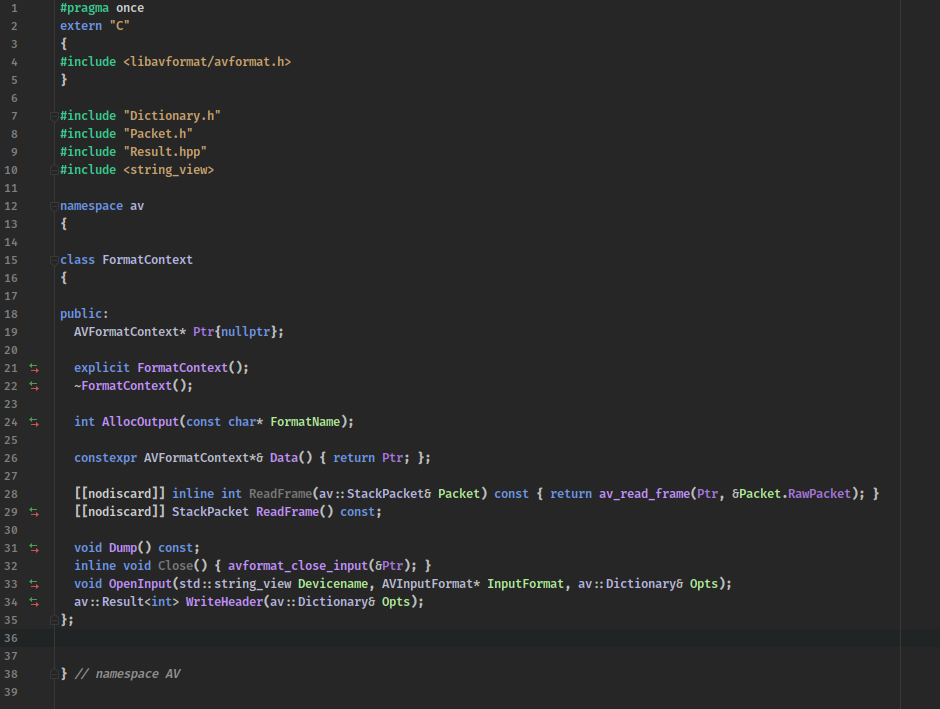
\includegraphics[width=\textwidth]{format_context_wrapper_header.png}
  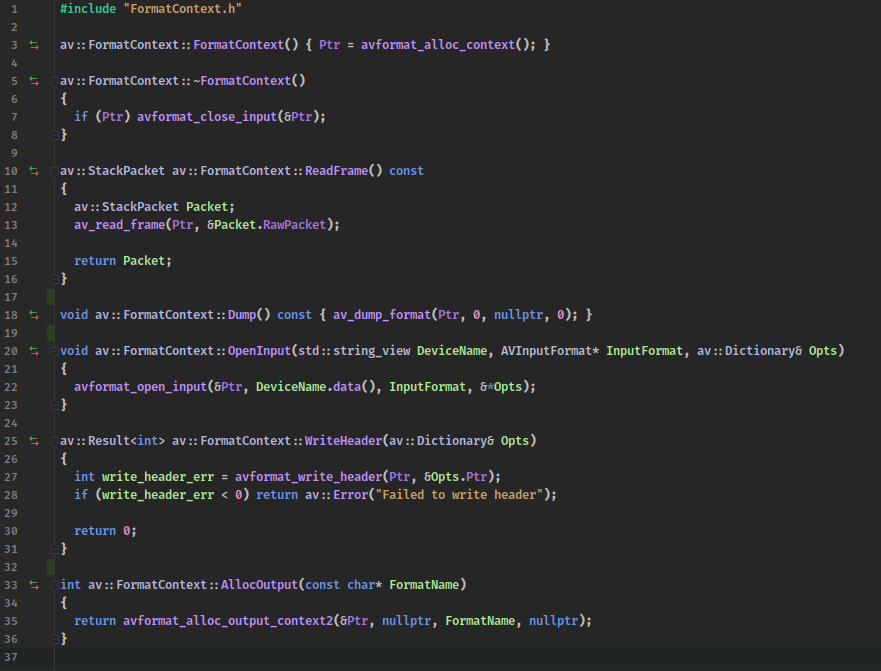
\includegraphics[width=\textwidth]{format_context_wrapper.png}
  \caption[Implementacija omotavajuće klase]{Implementacija omotavajuće klase oko strukture \keyword{AVFormatContext}}
\end{figure}
\clearpage

\myparagraph{Result} \label{sec:result}
Većina funkcija iz biblioteke, u pravom duhu programiranja u jeziku C, vrača kao rezultat kod tipa \keyword[p]{int} koji
je \textbf{negativan} ako se dogodila greška inače \textbf{0 ili pozitivan}. 
\\
Ovaj pristup je zastario i jako brzo dovodi do nepreglednog izvornog koda. Stoga su implementirane klase
\keyword{Result} i \keyword{Error} 
\\
\paraBreak
Klasa Error ima 3 polja: 
\begin{itemize}
  \item \keyword[p]{bool HasError} zastavica postavljena ako je došlo do greške
  \item \keyword[p]{int Code} vrijednost rezultata neke funkcije iz FFMpeg biblioteke.
  \item \keyword[p]{std::string Msg} predstavlja opis greške koja se dogodila u koliko se dogodila.
\end{itemize}
Radi pogodnosti ova klasa ima implementiran implicitni konstruktor koji prima \keyword[p]{int} (kod greške) i pomoću
FFMpeg funkcije \keyword[o]{av\_make\_error\_string} postavlja polje \keyword{Code}.
\paraBreak
Klasa Result je generična po parametru \keyword{T} i ima dva polja, 
\\ 
\keyword[p]{std::optional<T> \keyword{t}} i \keyword[p]{std::optional<Error> \keyword{error}}. 
\paraBreak
Polje t predstavlja stvarnu vrijednost koju klasa omotava i bit će postavljeno u slučaju da se greška nije dogodila,
inače je postavljeno polje error.
\paraBreak
Također implementira korisne metode za lakšu obradu slučaja u kojem se dogodila greška. 
\\
Metoda \keyword[o]{Unwrap} vrača vrijednost \keyword{T} ako nema greške, inače terminira program i ispisuje grešku. 
\\
Metoda \keyword[o]{UnwrapOr} prima parametar tipa \keyword{T} i vrača vrijednost \keyword{T} ako nema greške inače vrača
poslani parametar. 
\\
Metoda \keyword[o]{Expect} prima parametar tipa \keyword{std::string\_view} i vrača vrijednost \keyword{T} ako nema greške
inače terminira program i ispisuje poslani parametar kao poruku uz još i poruku originalne greške. 
\\
Metode \keyword[o]{HasError} i  \keyword[o]{HasData} pružaju lagan način za provjeravanje ako se dogodila greška.

\begin{figure}[h]
  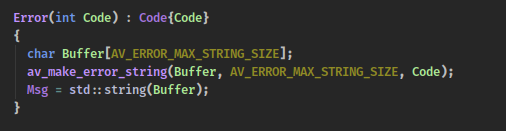
\includegraphics[width=\textwidth]{error_ctor.png}
  \caption[Konstruktor klase Error]{Konstruktor klase \keyword{Error}}
\end{figure}
\begin{figure}[h]
  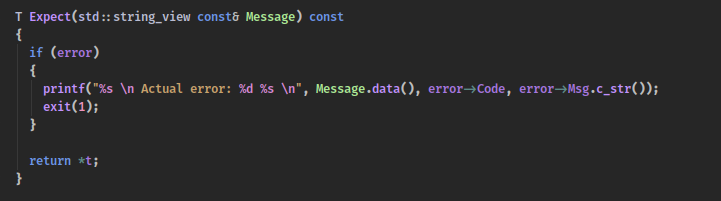
\includegraphics[width=\textwidth]{expect_impl.png}
  \caption[Klasa Result implementacija]{Implementacija metode \keyword[o]{Expect} klase Result}
\end{figure}
\begin{figure}[h]
  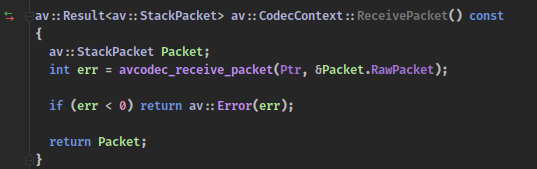
\includegraphics[width=\textwidth]{result_example1.png}
  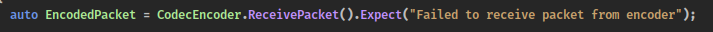
\includegraphics[width=\textwidth]{result_example2.png}
  \caption[Primjer korištenja klase Result]{Primjer korištenja klase \keyword{Result}}
\end{figure}


\clearpage
\subsubsection{FFmpeg strukture}
FFmpeg dolazi s ogromnim brojem struktura, od kojih velik dio nema veze sa samom manipulacijom videa,
u ovom poglavlju su opisane glavne strukture koji su korisne u tu svrhu.

% \clearpage
\myparagraph{AVInputFormat} \label{sec:input_format}
Struktura \keyword{AVInputFormat} sama po sebi nema velik značaj, predstavlja sposobnosti odabranog video upravljača, u
slučaju Raspberry pi-a jer je operativni sustav linux to je \hyperref[sct:v4l2]{\foreign{v4l2}}. \cite{ffmpegDocs} \cite{linuxKernelDocs}
\paraBreak
Dohvat ove strukture je tipično prvi korak i obavlja se pozivom funkcije \\
\keyword[o]{av\_find\_input\_format}, ona prima jedan parametar tipa \keyword[p]{const char*} koji predstavlja video upravljač.
\begin{figure}[h]
  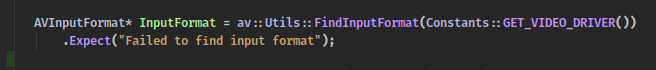
\includegraphics[width=\textwidth]{av_find_input_format2.png}
  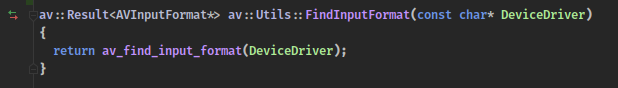
\includegraphics[width=\textwidth]{av_find_input_format.png}
  \begin{subfigure}{\textwidth}
    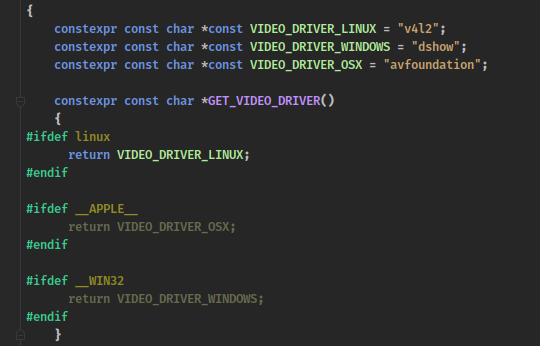
\includegraphics[width=\textwidth]{video_driver_constants.png}
    \caption{Primarni video upravljači na raznim platformama}
  \end{subfigure}
  \caption{Dohvat strukture AVInputFormat}
\end{figure}

\clearpage
\myparagraph{AVFormatContext} \label{sec:avformat_context}
Struktura \keyword{AVFormatContext} koja može biti ulazna ili izlazna služi za konfiguriranje ulaznog multimedijskog
uređaja ili datoteke, to jest ako je izlazna za konfiguriranje strukture i destinacije izlazne datoteke. 
\\
Primjerice sadrži sve struje (\keyword{AVStream}) podataka od izvora multimedije. U slučaju Raspberry pi kamere riječ je o samo
jednoj struji tipa video. \cite{ffmpegDocs}

\myparagraph{AVStream} \label{sec:avstream}
Struktura \keyword{AVStream} predstavlja struju podataka nekog izvora. 
\\
Ako imamo multimedijsku datoteku s videom i zvukom znači da ona sadrži dva \keyword{AVStream}-a jedan tipa Video i jedan
tipa Audio \cite{ffmpegDocs}
\begin{figure}[h]
  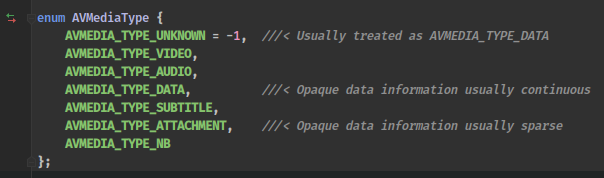
\includegraphics[width=\textwidth]{av_media_type.png}
  \caption[Enumeracija svih tipova media struja]{Enumeracija svih tipova media struja \cite{ffmpegDocs}}
\end{figure}

\myparagraph{AVCodec} \label{sec:avcodec}
Struktura \keyword{AVCodec} predstavlja kodek \ref{sec:codec}, može biti enkoder ili dekoder, ovisno o tipu kojeg želimo dohvaća se
funkcijama \keyword[o]{avcodec\_find\_encoder} ili 
\\ 
\keyword[o]{avcodec\_find\_decoder} svaka od kojih prima jedinstveni identifikator kodeka.
\paraBreak
Za svaki podržani kodek postoji jedna instance ove strukture i ona se nikad ne mijenja, za konfiguraciju samog kodeka
koristi se struktura \keyword{AVCodecContex}.

\begin{figure}[h]
  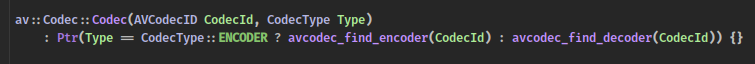
\includegraphics[width=\textwidth]{codec_ctor.png}
  \caption[Konstruktor Codec omotavajuće klase]{\small Konstruktor Codec omotavajuće klase koji ovisno o tipu kodeka zove odgovarajuću funkciju}
\end{figure}

\clearpage
  \begin{table}[h]
    \begin{minipage}{\textwidth}
      \tiny
      \centering
    \begin{tabular}{|c|c|c|}
      \hline
      Ime & Enkodiranje & Dekodiranje \\
      \hline
      AMV Video & - & X \\
      ANSI/ASCII art & - & X \\
      Apple Intermediate Codec & - & X \\
      Apple MJPEG-B & - & X \\
      Apple Pixlet & - & X \\
      Apple ProRes & X & X \\
      Apple QuickDraw & - & X \\
      Bink Video & - & X \\
      Bitmap Brothers JV video & - & X \\
      C93 video & - & X \\
      CamStudio & - & X \\
      CD+G & - & X \\
      CDXL & - & X \\
      Chinese AVS video & E & X \\
      Cinepak & X & X \\
      Cirrus Logic AccuPak & X & X \\
      Creative YUV (CYUV) & - & X \\
      DFA & - & X \\
      Dirac & E & E \\
      Dxtory capture format & - & X \\
      Flash Screen Video v2 & - & X \\
      Flash Video (FLV) & X & X \\
      FM Screen Capture Codec & - & X \\
      Forward Uncompressed & - & X \\
      Fraps & - & X \\
      H.261 & X & X \\
      H.263 / H.263-1996 & X & X \\
      H.263+ / H.263-1998 / H.263 version 2 & X & X \\
      H.264 / AVC / MPEG-4 AVC / MPEG-4 part 10 & E & X \\
      HEVC & X & X \\
      IBM Ultimotion & - & X \\
      Intel H.263 & - & X \\
      Intel Indeo * & - & X \\
      Interplay C93 & - & X \\
      Interplay MVE video & - & X \\
      Iterated Systems ClearVideo & - & X \\
      LOCO & - & X \\
      lossless MJPEG & X & X \\
      MagicYUV Lossless Video & - & X \\
      Microsoft ATC Screen & - & X \\
      MJPEG (Motion JPEG) & X & X \\
      Motion Pixels video & - & X \\
      MPEG-1 video & X & X \\
      MPEG-2 video & X & X \\
      MPEG-4 part 2 & X & X \\
      Nintendo Gamecube THP video & - & X \\
      NuppelVideo/RTjpeg & - & X \\
      VP8 & E & X \\
      VP9 & E & X \\
      planar RGB & - & X \\
      QuickTime 8BPS video & - & X \\
      QuickTime Animation (RLE) video & X & X \\
      QuickTime Graphics (SMC) & - & X \\
      QuickTime video (RPZA) & - & X \\
      R10K AJA Kona 10-bit RGB Codec & - & X \\
      R210 Quicktime Uncompressed RGB 10-bit & - & X \\
      Raw Video & X & X \\
      RealVideo 3.0 & - & X \\
      RealVideo 4.0 & - & X \\
      Renderware TXD (TeXture Dictionary) & - & X \\
      RL2 video & - & X \\
      Sierra VMD video & - & X \\
      Silicon Graphics RLE 8-bit video & - & X \\
      Theora & E & X \\
      Tiertex Limited SEQ video & - & X \\
      Ut Video & X & X \\
      v210 QuickTime uncompressed 4:2:2 10-bit & X & X \\
      Windows Media Video 8 & X & X \\
      Windows Media Video 9 & - & X \\
      Wing Commander III / Xan & - & X \\
      Wing Commander IV / Xan & - & X \\
      WMV7 & X & X \\
      YAMAHA SMAF & X & X \\
      ZLIB & X & X \\
      \hline
    \end{tabular}
    \caption[Neki od podržanih kodeka biblioteke FFMpeg]
    {\small Neki od podržanih kodeka biblioteke FFMpeg \cite{ffmpegBook}}
    \footnotetext{\tiny \textbf{E} predstavlja podršku uz vanjsku biblioteku}
  \end{minipage}
\end{table}

  

\clearpage
\myparagraph{AVCodecContext} \label{sec:avcodec_context}
Struktura \keyword{AVCodecContext} služi kao kontejner kodeka, skroz ovu strukturu se podešavaju sve postavke kodeka
kao što su broj slika u sekundi, visina slike, širina slike i mnoge druge ovisno o samom kodeku. \\
Sve funkcije vezane za dekodiranje ili enkodiranje primaju ovu strukturu kao prvi parametar te ovisno o postavkama iste,
enkodiraju ili dekodiraju slike na određeni način.

\myparagraph{AVIOContext} \label{sec:aviocontext}
Struktura \keyword{AVIOContext} dio je izlaznog \keyword{AVFormatContext}-a i predstavlja finalno odredište enkodiranih
paketa, u slučaju ovoga rada to je TCP poslužitelj ali može biti i putanja na disku ili neki drugi mrežni protokol.

\myparagraph{AVFrame} \label{sec:av_frame}
Struktura \keyword{AVFrame} predstavlja jednu dekodiranu sliku videa. 
\\
Ovu strukturu dekoder vrača nakon dekodiranja, te ju isto tako enkoder prima kao parametar. \cite{ffmpegDocs}
\paraBreak
Ima velik broj polja, naj važniji od kojih su:
\begin{itemize}
  \item \keyword[p]{int width, height} predstavljaju visinu i širinu slike.
  \item \keyword[p]{int64\_t pts} prezentacijska vremenska oznaka, odnosno vrijeme relativno u odnosu na ostale slike, kada se ova
  slika treba prikazati. Ovaj parametar postaje ključan kod enkodiranja jer se mora računati za svaku enkodiranu sliku i o njemu
  ovisi ispravnost prikaza slika. \cite{ffmpegDocs} \\
  Kod dekodirane slike dovoljno je ovo polje samo inkrementirati, te nakon enkodiranja ga korektno postaviti.
  \item \keyword[p]{pict\_type} predstavlja tip slike \ref{sec:slika}
  \item \keyword[p]{data} pokazivač na ravnine slika. \ref{sec:planar}
  \item \keyword[p]{linesize} veličina svake od ravnina slike u bajtovima. \ref{sec:planar}
\end{itemize}

\myparagraph{AVPacket} \label{sec:av_packet}
Struktura \keyword{AVPacket} predstavlja enkodirani paket, odnosno jednu enkodiranu sliku videa. \\
Ova struktura dobiva se kao rezultat enkodiranja slike i šalje se na odredišnu lokaciju specificiranu kroz 
\keyword{AVIOContext} strukturu \ref{sec:aviocontext} \\

\myparagraph{SwsContext} \label{sec:sws_context}
Struktura \keyword{SwsContext} služi za razne manipulacije pojedinačnim slikama videa, naj bitnije, funkcija
\keyword[o]{sws\_scale} kojom je moguće promijeniti piksel format ili veličinu/širinu slike. \\
Za instanciranje koristi se funkcija \keyword[o]{sws\_getContext} koja prima izvornu visinu i širinu i izvorni
piksel format, te proizvoljne odredišne iste parametre, zatim raznim vezanim funkcijama radi pretvorbe.

\myparagraph{AVRational} \label{sec:av_rational}
Struktura \keyword{AVRational} predstavlja razlomak, ima dva polja \keyword[p]{num} i \keyword[p]{den}, num ili numerator
je brojnik a den ili denumerator je djelitelj.
\paraBreak
Ova struktura se koristi za razne postavke kao što su broj slika u sekundi, primjerice ako želimo \keyword{AVCodecContext}-u
postaviti broj slika u sekundi na 30 to bi napravili kao \keyword{AVRational} gdje num ima vrijednost 30 a den 1 što efektivno
znaci 30 / 1 odnosno 30.
\paraBreak
FFMpeg koristi ovakvu strukturu a ne \keyword[p]{float} brojeve jer su operacije nad \keyword[p]{float} brojevima gubitačne
i ne potpuno precizne ovisno o broju decimala a priroda nekih od dijelova procesa enkodiranja zahtjeva izrazito 
točne kalkulacije. \cite{ffmpegDocs}

\myparagraph{AVDictionary}
Struktura \keyword{AVDictionary} predstavlja ključ - vrijednost mapu implementiranu u jeziku C. Ona se koristi za
prosljeđivanje većine postavki ostalih struktura.

\clearpage
\subsubsection{Konfiguracija}\label{sec:configuration}
Konfiguracija transkodera je prilično jednostavna. \\
Očekuje konfiguracijsku \foreign{JSON} datoteku imena cfg.json u istom direktoriju kao i sami izvršni program, ili ako je
riječ o operativnom sustavu \foreign{linux} i nije našao datoteku cfg.json pogledati u putanji \foreign{/etc/hst/cfg.json}
\paraBreak
Za parsiranje JSON datoteke koristi se biblioteka \foreign{nlohmann json} \cite{nlohmanJson}
\paraBreak
Postavke korisničke konfiguracije predstavlja klasa \keyword{Configuration} i sadrži polja:
\begin{itemize}
  \item \keyword[o]{int Width} - širina slike
  \item \keyword[o]{int Height} - visina slike
  \item \keyword[o]{int Framerate} - broj slika u sekundi
  \item \keyword[o]{std::string DeviceName} - ime uređaja koje će se prikazati na klijentima
  \item \keyword[o]{std::string ServerIp} - IP TCP poslužitelja
  \item \keyword[o]{std::string ServerPort} - Port TCP poslužitelja
\end{itemize}

\begin{figure}[h]
  \centering
  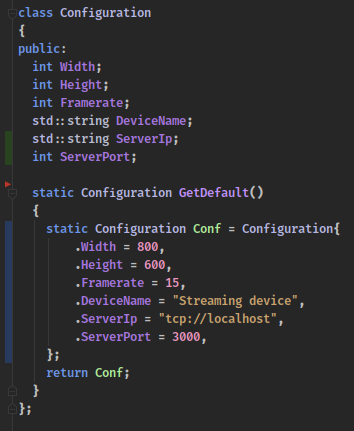
\includegraphics[height=10cm, keepaspectratio]{transcoder_configuration.png}
  \caption{Klasa Configuration}
\end{figure}
\clearpage
\begin{figure}[h]
  \centering
  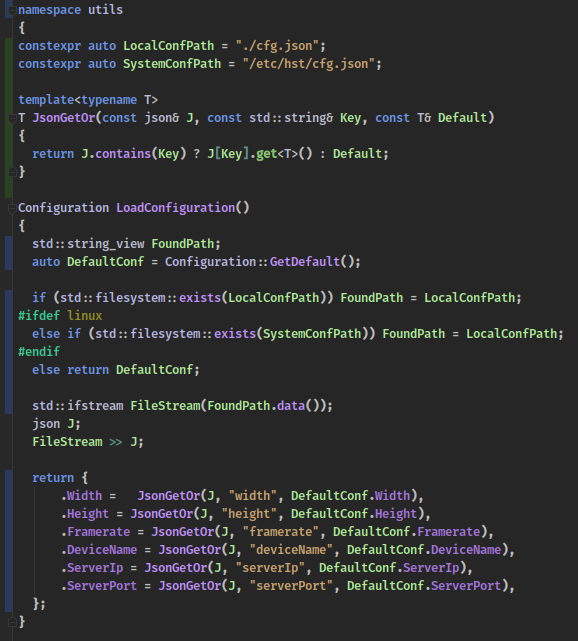
\includegraphics[width=\textwidth,height=\textheight,keepaspectratio]{parse_configuration.png}
  \caption{Parsiranje konfiguracijske datoteke}
\end{figure}
\clearpage

\subsubsection{Pristup kameri}
Da bi mogli početi primati slike iz kamere prvo moramo pronaći lokaciju iste, na \foreign{linux} operativnom sustavu
primjer lokacije bio bi \foreign{/dev/video0}
\paraBreak
U ovu svrhu FFMpeg \ref{sec:ffmpeg} nudi pomočnu funkciju \keyword[o]{avdevice\_list\_input\_sources} koja kao parametar
prima \keyword{AVInputFormat} \ref{sec:input_format} i vrača listu svih ulaznih multimedijskih uređaja u sustavu.
\paraBreak

\begin{figure}[h]
  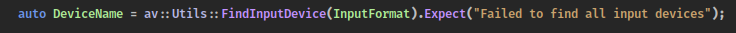
\includegraphics[width=\textwidth]{find_device1.png}
  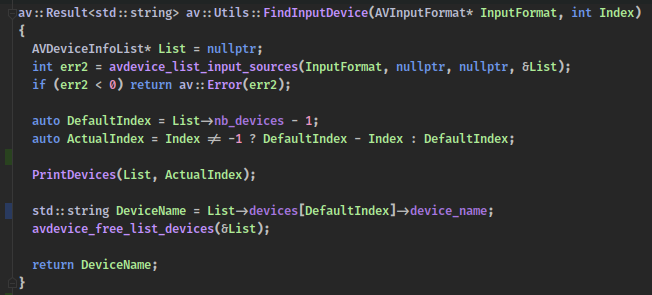
\includegraphics[width=\textwidth]{find_device2.png}
  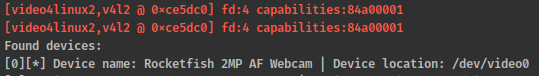
\includegraphics[width=\textwidth]{found_device_log.png}
  \caption{Dohvaćanje lokacije ulaznog uređaja}
\end{figure}

\subsubsection{Čitanje i dekodiranje paketa iz kamere}
\myparagraph{Otvaranje ulaznog formata}
Za čitanje podataka iz kamere potreban nam je ulazni \keyword{AVFormatContext} \ref{sec:avformat_context} koji se alocira funkcijom 
\keyword[o]{avformat\_alloc\_context} te se zatim otvara funkcijom \\
\keyword[o]{avformat\_open\_input} koja prima lokaciju uređaja  i video upravljač, te postavke same slike koja dolazi
iz kamere, visina, širina te broj slika u sekundi.
Ove postavke uzimaju se iz konfiguracijske datoteke.\ref{sec:configuration}
\paraBreak
Sami izvorni format sada sadrži polje struja podataka \keyword{AVStream}, u slučaju Raspberry pi kamere samo jednu struju
tipa Video ali kada bi otvarali tipični film na ovaj način to polje bi o barem dvije struje 
\footnote{Ne nužno, u slučaju da video nema zvuk}, jednu tipa Video i jednu tipa Audio, te potencijalno i tipa Titlovi.

\begin{figure}[h]
  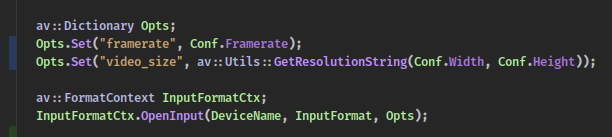
\includegraphics[width=\textwidth]{format_open_input.png}
  \caption{Otvaranja ulaznog formata}
\end{figure}

\myparagraph{Konfiguracija dekodera}
Nakon otvaranja ulaznog formata možemo funkcijom \keyword[o]{av\_read\_frame} čitati iz kamere, iako se zove 
\foreign{read\_frame} ona ne vrača slike nego pakete \ref{sec:av_packet} enkodirane \foreign{RAW\_VIDEO} kodekom taj
kodek označava da slika sadrži čiste podatke koje nije moguće prikazati na ekranu. \cite{ffmpegBook}
\paraBreak
Ovakvi paketi nisu korisni jer nisu čitljivi od strane video playera, a uz to su ogromne veličine, primjerice za sliku
veličine 1280x1024 veličina jednog paketa je 2621440 bajtova, odnosno 2.62 megabajta, za video koji se vrti
na 24 slike u sekundi to je \textbf{40MB} po \textbf{sekundi} videa.\

\begin{figure}[h]
  \centering
  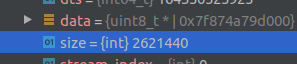
\includegraphics[width=0.5\textwidth]{raw_packet_size.png}
  \caption{\small Veličina \foreign{raw} paketa iz kamere}
\end{figure}
\noindent
Zato ih se prvo mora dekodirati u čiste slike \ref{sec:av_frame}, pa zatim enkodirati nekim drugim kodekom, 
u slučaju ovog rada to je \foreign{VP9} kodek.
\paraBreak
Konfiguracija samog dekodera koji je u biti struktura \keyword{AVCodecContext} \ref{sec:avcodec_context} je
jednostavna, sve postavke se kopiraju iz ulaznog izvora koji se nalazi u ulaznom \keyword{AVFormatContext}-u funkcijom
\keyword[o]{avcodec\_parameters\_to\_context}, on u sebi već sadrži sve potrebne informacije o kodeku.
\\
Nakon konfiguracije zove se funkcija \keyword[o]{avcodec\_open2}.
\clearpage

\begin{figure}[h]
  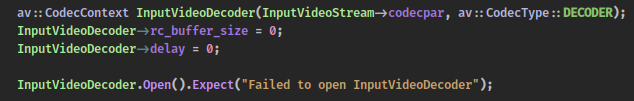
\includegraphics[width=\textwidth]{decoder_conf.png}
  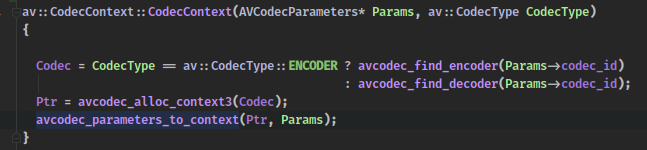
\includegraphics[width=\textwidth]{decoder_conf2.png}
  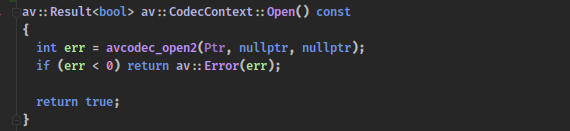
\includegraphics[width=\textwidth]{open_codec_context.png}
  \caption{Konfiguriranje i otvaranje dekodera}
\end{figure}
\noindent
Nakon čitanja paketa iz kamere ovim dekoderom ih možemo dekodirati u slike, tako da prvo pošaljemo paket u
dekoder funkcijom \keyword[o]{avcodec\_send\_packet} te funkcijom \keyword[o]{avcodec\_receive\_frame} nazad dobivamo 
dekodiranu sliku.
\begin{figure}[h]
  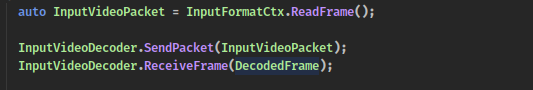
\includegraphics[width=\textwidth]{decoding_example.png}
  \caption{Dekodiranje paketa iz kamere}
\end{figure}

\begin{figure}[h]
  \centering
  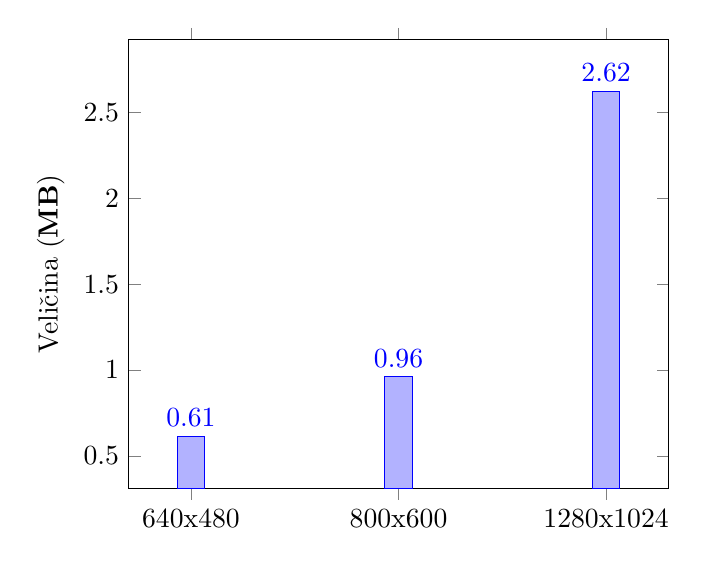
\begin{tikzpicture}
    \begin{axis}[
      ybar,
      enlargelimits=0.15,
      legend style={at={(0.5,-0.15)},
        anchor=north,legend columns=-1},
      ylabel={Veličina (\textbf{MB})},
      symbolic x coords={640x480,800x600,1280x1024},
      xtick=data,
      nodes near coords,
      nodes near coords align={vertical},
      ]
    \addplot coordinates {(640x480,0.614) (800x600, 0.96) (1280x1024, 2.6214)};
    \end{axis}
  \end{tikzpicture}
  \caption{Graf veličine \foreign{raw} paketa iz kamere na raznim rezolucijama} \label{pic:packet_size}
\end{figure}
\clearpage


\subsubsection{Enkodiranje slika} \label{sec:encoding}
\myparagraph{Konfiguracija enkodera}
Da bi se enkoder konfigurirao prvo se mora znati o kojem je riječ, za ovu svrhu postoji enumeracija \keyword{AVCodecID} \cite{ffmpegDocs}
koja predstavlja jedinstveni identifikator svakog od podržanih kodeka.
\begin{figure}[h]
  \centering
  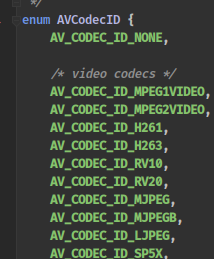
\includegraphics[width=0.33\textwidth, height = 5cm]{avcodec_id_enum.png}
  \caption{\small Enumeracija jedinstvenih identifikatora kodeka}
\end{figure}
\paraBreak
Za dohvat \foreign{VP9} kodeka koristi se vrijednost \keyword[p]{AV\_CODEC\_ID\_VP9}, pozivom funkcije \keyword[o]{avcodec\_find\_encoder}
koja prima identifikator kao parametar. \\
S uspješno pronađenim kodekom se instacira struktura \keyword{AVCodecContext} \ref{sec:avcodec_context} pozivom funkcije
\keyword[o]{avcodec\_alloc\_context3} preko koje se konfigurira sami kodek.

\begin{figure} [h]
  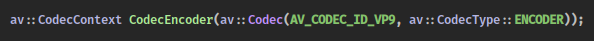
\includegraphics[width=\textwidth]{encoder1.png}
  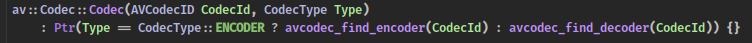
\includegraphics[width=\textwidth]{encoder2.png}
  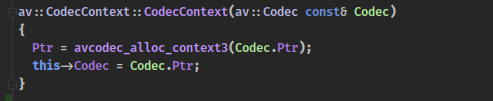
\includegraphics[width=\textwidth]{encoder3.png}
  \caption{Instanciranje kodek konteksta}
\end{figure}
\noindent
Nad samim kodekom moguće je podesiti ogroman broj postavki, najbitnije od kojih su: 
\begin{itemize}
  \item \keyword[p]{width}, \keyword[p]{height} - očekivana visina i širina pojedinačne slike
  \item \keyword[p]{time\_base} - glavna jedinica vremena u sekundama na osnovu koje su vremenske oznake slike 
    predstavljene. Za video fiksnog broja slika u sekundi ovaj parametar se postavlja na invertnu vrijednost broja slika u sekundi. \\
    Recimo da je broj slika u sekundi 15 odnosno 15/1, tada je \foreign{time\_base} 1/15. \\
    Kontejneri često forsiraju fiksan \foreign{time\_base}
  \item \keyword[p]{gob\_size} - \foreign{gob} ili \foreign{group of pictures size} predstavlja koliko će enkoder proizvest
   P slika za svaku I sliku \ref{sec:slika}
  \item \keyword[p]{max\_b\_frames} - Maksimalan dopušteni broj B slika \ref{sec:slika}, u slučaju živog prijenosa postavljen na 0
   jer iako B slike smanjuju konačnu veličinu, isto tako drastično povećavaju kašnjenje slike.
  \item \keyword[p]{thread\_count} - Broj dretvi koje će enkoder interno koristiti za enkodiranje.
  \item \keyword[p]{pix\_fmt} - Odredišni piksel format, u slučaju \foreign{VP9} kodeka \\ mora biti planaran \ref{sec:pixelformat}.
  \item \keyword[p]{bit\_rate} - broj procesiranih bitova u jedinici vremena, ovaj parametar drastično utječe na kvalitetu
    i veličinu finalne slike. Veća vrijednost znači bolja slika ali isto tako i veća slika.
  \item \keyword[p]{crf} - \foreign{crf} ili \foreign{Constant Rate Factor} se odnosi na varijabilni \foreign{bit\_rate}
    odnosno enkoder pokušava održavati konzistentnu kvalitetu slike i sukladno time sam odlučuje o vrijednosti 
    \foreign{bit\_rate}-a. \\
    Podržane vrijednosti ovise do kodeka, u slučaju \foreign{VP9} 0-63, neovisno o kodeku doduše,
    manja vrijednost predstavlja bolju sliku uz veći prosječni \foreign{bit\_rate}
\end{itemize}

\begin{figure}[h]
  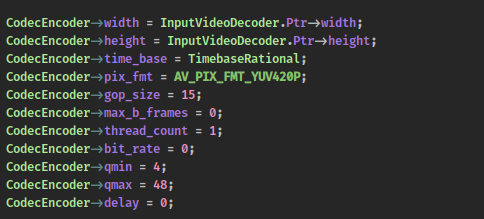
\includegraphics[width=\textwidth]{encoder_configuration.png}
  \caption{Konfiguracija enkodera}
\end{figure}
\noindent
Prije nego se dobivena slika \footnote{Slika dobivena od dekodera} može enkodirati, mora joj se promijeniti piksel format. \\
\foreign{VP9} enkoder zahtjeva \foreign{planarni} \ref{sec:slika} piksel format što piksel format slike dobivene iz 
kamere nije. \\
Ovaj proces zahtjeva prilično ne jasnu matematiku, srećom FFMpeg \ref{sec:ffmpeg} nudi pomočnu
funkciju \keyword[o]{sws\_scale} upravo za tu svrhu, osim piksel formata može skalirati visinu ili širinu slike. \\
Prvo je potrebno instancirati strukturu \keyword{SwsContext} \ref{sec:sws_context}, funkcijom \keyword[o]{sws\_getContext}
koja prima izvorni piksel format odnosno onaj iz kojeg pretvaramo te odredišni odnosno onaj u kojeg pretvaramo.

\begin{figure}[h]
  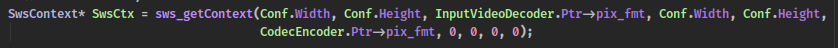
\includegraphics[width=\textwidth]{scale1.png}
  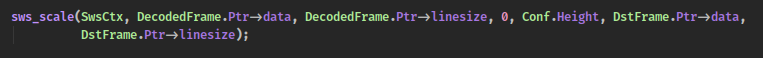
\includegraphics[width=\textwidth]{scale2.png}
  \caption{Promjena piksel formata slike}
\end{figure}
\noindent
Prije samog enkodiranja još je potrebno postaviti prezentacijsku vremensku oznaku \ref{sec:av_frame} dekodirane slike,
ovaj korak je potreban samo ako je izvor kamera jer te slike iz očitih razloga ovo polje nemaju postavljeno, zasad ju je
dovoljno samo inkrementirati za svaku dobivenu sliku počevši od nule.
\paraBreak
Enkodiranje se izvodi slično kao dekodiranje samo s obrnutim parametrima, prvo se nad enkoderom zove funkcija
\keyword[o]{avcodec\_send\_frame} koja prima dekodiranu sliku, zatim funkcija \keyword[o]{avcodec\_receive\_packet} koja 
vrača enkodirani paket.

\begin{figure}[h]
  
\includegraphics[width=\textwidth]{encoding1.png}
  
\includegraphics[width=\textwidth]{encoding2.png}
  \caption{Enkodiranje slike}
\end{figure}
\noindent
Rezultat enkodiranja je slika znatno manje veličine, primjerice paket koji je došao iz kamere veličine 
\textbf{0.96 MB} sada je velik samo \textbf{10-20 KB}, što je nevjerojatna razlika.\\
Međutim ta vrijednost predstavlja I sliku \ref{sec:slika}, koja se pojavljuje \footnote{Ovisno o konfiguraciji} svakih 15
paketa, P slika s druge strane je još znatno manja te varira između \textbf{100 B} do \textbf{5 KB} ovisno o količini
kretnje u slici. \\
Ako ove vrijednosti usporedimo s primjerom navedenim u \ref{sec:size_problem} konačna veličina bila bi otprilike 
\textbf{71 MB} u usporedbi sa \textbf{62.2 GB}

\clearpage

\begin{figure}
  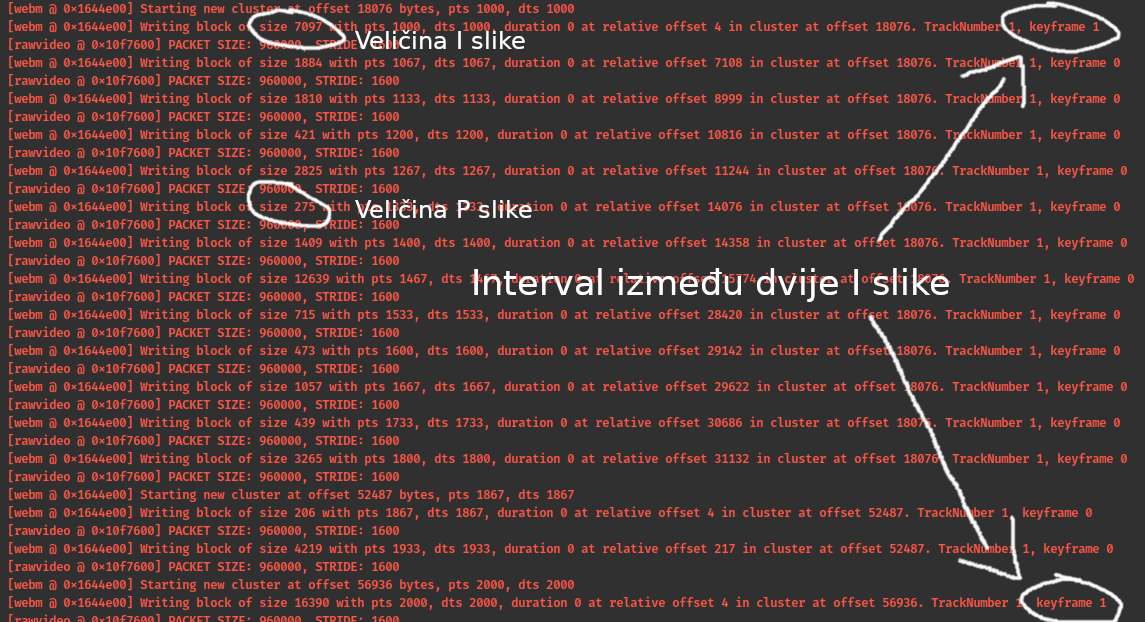
\includegraphics[width=\textwidth, height=15cm]{keyframes.png}
  \caption{Ispis kodeka}
\end{figure}

\begin{center}
  \begin{table}[h]
    \begin{tabular}{|c|c|c|c|}
      \hline
      Rezolucija & Paket iz kamere & Enkodirani paket, I slika & Enkodirani paket, P slika \\
      \hline
      640x480 & 614400 & 13497 & 1781 \\[0.5cm]
      800x600 & 960000 & 14409 & 1821 \\[0.5cm]
      1280x1024 & 2621440 & 26066 & 3286 \\[0.5cm]
      \hline
    \end{tabular}
    \caption[Usporedba veličina paketa prije i poslije enkodiranja]{Usporedba veličina paketa prije i poslije enkodiranja u \textbf{bajtovima}}
\end{table}
\end{center}

\begin{figure}[h]
  \centering
  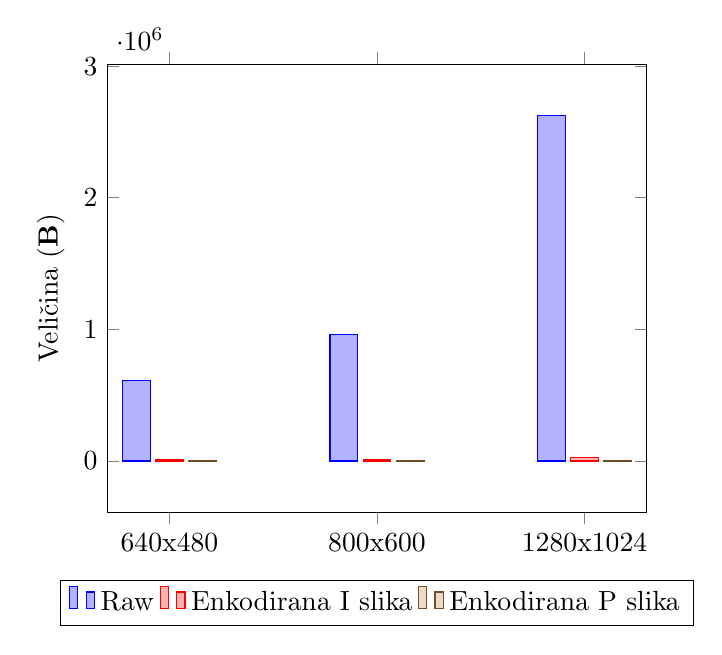
\begin{tikzpicture}
    \begin{axis}[
      ybar,
      enlargelimits=0.15,
      legend style={at={(0.5,-0.15)},
        anchor=north,legend columns=-1},
      ylabel={Veličina (\textbf{B})},
      symbolic x coords={640x480,800x600,1280x1024},
      xtick=data,
      nodes near coords align={vertical},
      ]
    \addplot coordinates {(640x480,614400) (800x600, 960000) (1280x1024, 2621440)};
    \addplot coordinates {(640x480,13497) (800x600, 14409) (1280x1024, 26066)};
    \addplot coordinates {(640x480,1781) (800x600, 1821) (1280x1024, 3286)};
    \legend{Raw, Enkodirana I slika, Enkodirana P slika}
    \end{axis}
  \end{tikzpicture}
  \caption[Graf usporedbe veličina paketa prije i poslije enkodiranja]{Graf usporedbe veličina paketa prije i poslije enkodiranja u \textbf{bajtovima}} \label{pic:packet_size}
\end{figure}

\begin{figure}[h]
  \centering
  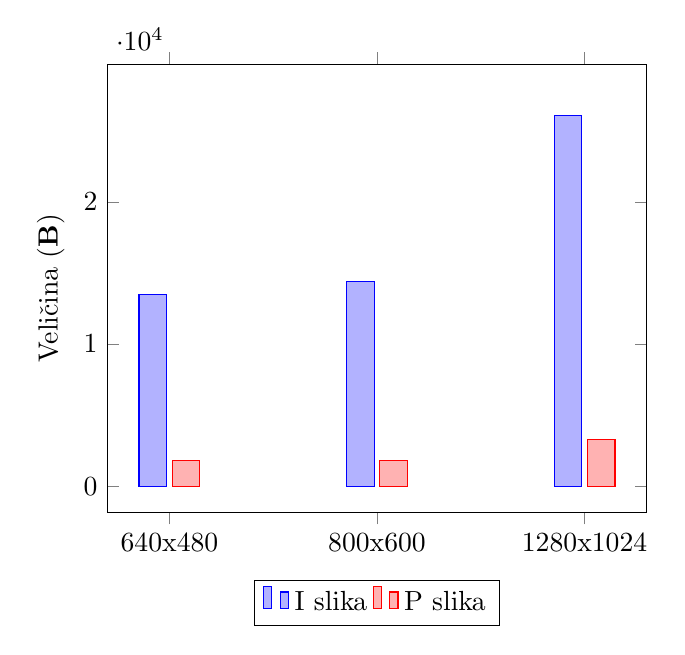
\begin{tikzpicture}
    \begin{axis}[
      ybar,
      enlargelimits=0.15,
      legend style={at={(0.5,-0.15)},
        anchor=north,legend columns=-1},
      ylabel={Veličina (\textbf{B})},
      symbolic x coords={640x480,800x600,1280x1024},
      xtick=data,
      nodes near coords align={vertical},
      ]
    \addplot coordinates {(640x480,13497) (800x600, 14409) (1280x1024, 26066)};
    \addplot coordinates {(640x480,1781) (800x600, 1821) (1280x1024, 3286)};
    \legend{I slika, P slika}
    \end{axis}
  \end{tikzpicture}
  \caption[Graf usporedbe veličina I i P slika]{Graf usporedbe veličina I te P slika u \textbf{bajtovima}} \label{pic:pict_type}
\end{figure}
\clearpage

\clearpage
\subsubsection{Slanje enkodiranih paketa kroz mrežu}
\myparagraph{Konfiguracija izlaznog formata}
Izlazni format se konfigurira kroz strukturu \keyword{AVFormatContext} \ref{sec:avformat_context}, potrebno ju je
alocirati funkcijom \keyword[o]{avformat\_alloc\_context} koja se automatski poziva kao dio konstruktora omotavajuće
klase \ref{sec:libav_wrappers}
\paraBreak
Ova struktura ima polje tipa \keyword{AVOutputFormat} koje opisuje format i karakteristike izlazne datoteke,
naj bitnije kontejner \ref{sec:container},
u slučaju ovog rada to je \foreign{WebM},
\\
Alocira se funkcijom \keyword[o]{avformat\_alloc\_output\_context2} koja prima naziv ili kraticu formata.
\paraBreak
Zadnje polje koje se mora postaviti je \keyword{pb} predstavljeno \\
strukturom \keyword{AVIOContext} \ref{sec:aviocontext}, ovdje postavljamo konačno odredište odnosno adresu poslužitelja, ali
isto tako može biti i putanja na disku.
\begin{figure}[h]
  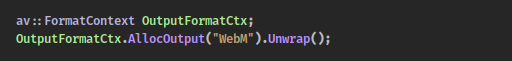
\includegraphics[width=\textwidth]{outputformat_alloc1.png}
  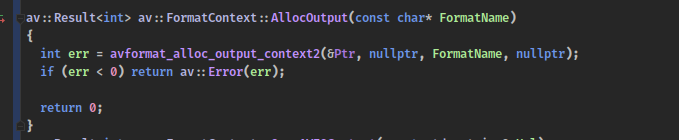
\includegraphics[width=\textwidth]{outputformat_alloc2.png}
  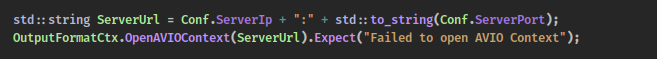
\includegraphics[width=\textwidth]{outputformat_alloc3.png}
  \caption[Kreiranje izlaznog formata]{Kreiranje izlaznog formata te specificiranje kontejnera i odredišta}
\end{figure}

\myparagraph{Konfiguracija izlaznog video toka}\label{sec:output_format_ctx}
Video tok ili struju podataka predstavlja struktura \keyword{AVStream} \ref{sec:avstream}, u slučaju Raspberry pi kamere
potreban samo jedan tok tipa Video, ako bi se htio imati zvuk preko recimo mikrofona jednostavno se doda još jedan tok
tipa Audio, te ih se na kraju \foreign{mux}-a zajedno.
\paraBreak
Video tok se kreira pozivom funkcije \keyword[o]{avformat\_new\_stream} koja prima izlazni format te enkoder iz kojih
kopira sve potrebne parametre. \\
Po tim parametrima video player-i ali i bilo koji drugi čitači datoteka znaju o kakvoj je datoteci riječ te kakve su joj
karakteristike.
\paraBreak
Konačno funkcija \keyword[o]{avformat\_write\_header} zapisuje sve postavljene podatke u zaglavlje datoteke, odnosnu u slučaju
kada je odredište adresa poslužitelja, šalje to zaglavlje kroz mrežu. \\
Zaglavlje je izuzetno bitno jer bez njega nije moguće prikazati video, player ne bi znao o kojem je kontejneru riječ, kojim
je kodekom slika enkodirana, kojom brzinom se video vrti itd. \\
Sam FFMpeg \ref{sec:ffmpeg}, ne dozvoljava slanje paketa prije nego se zapiše poglavlje, jer zbog spomenutih razloga to ni
nema smisla. \cite{ffmpegDocs}

\begin{figure}[h]
  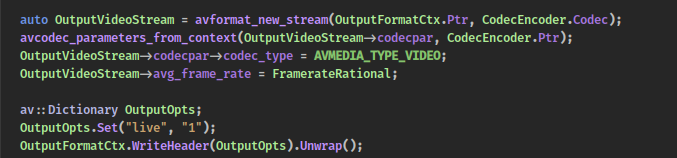
\includegraphics[width=\textwidth]{outputstream_write_header.png}
  \caption{Konfiguracija izlaznog toka te zapisivanje zaglavlja}
\end{figure}

\begin{figure}[h]
  \centering
  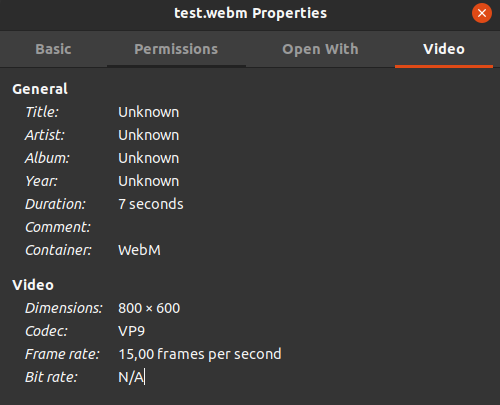
\includegraphics[width=0.75\textwidth]{video_details.png}
  \caption{Ispravno zapisano zaglavlje datoteke}
\end{figure}

\clearpage
\myparagraph{Slanje}
Prije samog slanja enkodiranih paketa moraju im se promijeniti prezentacijske vremenske oznake \ref{sec:av_frame}, u
suprotnom će prikaz videa biti pre brz ili pre spor.
\paraBreak
Do ovoga dolazi jer kontejneri forsiraju određeni \foreign{time\_base} \ref{sec:encoding}, primjerice kontejner WebM ima
fiksan \foreign{time\_base} 1/1000, \cite{ffmpegBook} dok izlazni format ima \\ 
\colorbox{gray}{1 / broj slika u sekundi}.  Zbog ovog dolazi  do pre brzog prikaza slika odnosno pre sporog ako je broj
slika u sekundi veći od 1000 ako se prezentacijske oznake ne usklade.
\paraBreak
Usklađivanje prezentacijskih oznaka se radi funkcijom \keyword[o]{av\_rescale\_q}, ona prima \foreign{time\_base} enkodera
i \foreign{time\_base} odredišnog video toka te vrača korektnu vrijednost prezentacijske oznake.
\begin{figure}[h]
  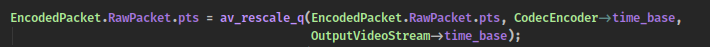
\includegraphics[width=\textwidth]{pts_sync.png}
  \caption{Usklađivanje prezentacijskih oznaka}
\end{figure}
\noindent
Nakon dobro postavljenih prezentacijskih oznaka enkodirani paket se šalje na odredište određeno izlaznim formatom
funkcijom \keyword[o]{av\_interleaved\_write\_frame}
\begin{figure}[h]
  
\includegraphics[width=\textwidth]{write_frame1.png}
  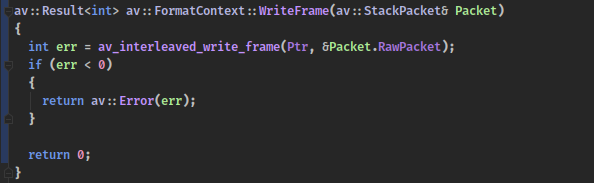
\includegraphics[width=\textwidth]{write_frame2.png}
  \caption{Slanje enkodiranih paketa}
\end{figure}